\documentclass[10pt]{beamer}

\usepackage[utf8x]{inputenc}
\usepackage[T1]{fontenc}
\usepackage{lmodern}
\usepackage{microtype}
\usepackage{xspace}
\usepackage[binary-units=true]{siunitx}
\usepackage{graphicx}
\usepackage{hyperref}
\usepackage{todonotes}
\usepackage{epstopdf}
\usepackage{array}
\usepackage{multicol}
\usepackage{multirow}
\usepackage{tabularx} % tabular with automatic line-break
\newcolumntype{Y}{>{\centering\arraybackslash}X} % centered column
\usepackage{amsmath}
\usepackage{grffile} % better name handling with graphicx
\usepackage{currfile} % provides relative file inclusion for tikzscale

\usepackage{tikz}
\usepackage{pgfplots}
\usepackage{pgfplots}
\usepackage{tikzscale}
\pgfplotsset{compat=newest}
\usetikzlibrary{plotmarks}
\usepackage{rotating}
\usepackage[absolute,overlay]{textpos}
\usepackage{circuitikz}

% Math symbols
\usepackage{amsmath}
\usepackage{amssymb}
\usepackage{amsthm}
\DeclareMathOperator*{\argmin}{arg\,min}
\DeclareMathOperator*{\argmax}{arg\,max}
\newcommand\norm[1]{\left\lVert#1\right\rVert}

% Sets
\newcommand{\Z}{\mathbb{Z}}
\newcommand{\R}{\mathbb{R}}
\newcommand{\Rn}{\R^n}
\newcommand{\Rnn}{\R^{n \times n}}
\newcommand{\C}{\mathbb{C}}
\newcommand{\K}{\mathbb{K}}
\newcommand{\Kn}{\K^n}
\newcommand{\Knn}{\K^{n \times n}}

% Unit vectors
\usepackage{esint}
\usepackage{esvect}
\newcommand{\kmath}{k}
\newcommand{\xunit}{\hat{\imath}}
\newcommand{\yunit}{\hat{\jmath}}
\newcommand{\zunit}{\hat{\kmath}}
\newcommand{\uunit}{\hat{\umath}}

% rot & div & grad & lap
\DeclareMathOperator{\newdiv}{div}
\newcommand{\divn}[1]{\nabla \cdot #1}
\newcommand{\rotn}[1]{\nabla \times #1}
\newcommand{\grad}[1]{\nabla #1}
\newcommand{\gradn}[1]{\nabla #1}
\newcommand{\lap}[1]{\nabla^2 #1}

% Elec
\newcommand{\B}{\vec B}
\newcommand{\E}{\vec E}
\newcommand{\EMF}{\mathcal{E}}
\newcommand{\perm}{\varepsilon} % permittivity

\newcommand{\bigoh}{\mathcal{O}}
\newcommand\eqdef{\triangleq}

\DeclareMathOperator{\newdiff}{d} % use \dif instead
\newcommand{\dif}{\newdiff\!}
\newcommand{\fpart}[2]{\frac{\partial #1}{\partial #2}}
\newcommand{\ffpart}[2]{\frac{\partial^2 #1}{\partial #2^2}}
\newcommand{\fdpart}[3]{\frac{\partial^2 #1}{\partial #2\partial #3}}
\newcommand{\fdif}[2]{\frac{\dif #1}{\dif #2}}
\newcommand{\ffdif}[2]{\frac{\dif^2 #1}{\dif #2^2}}
\newcommand{\constant}{\ensuremath{\mathrm{cst}}}

\newcommand{\dx}{\dot{x}}
\newcommand{\dy}{\dot{y}}
\newcommand{\ds}{\dot{s}}
\newcommand{\db}{\dot{b}}

\usepackage{comment}
\usepackage{pgfpages}
\usepackage{bm}

\usetheme[progressbar=frametitle]{metropolis}
\tikzset{font={\fontsize{10pt}{12}\selectfont}}

\usepackage{booktabs}
\usepgfplotslibrary{dateplot}

\usepackage{xspace}
\usepackage{bm}
\newcommand{\subfigwidth}{0.48\textwidth}
\usepackage{amsmath}
\usepackage{mathtools}

\title{LINMA2361 - Nonlinear dynamical systems}
\subtitle{Language dynamics}
\date{January 8, 2018}
\author{Quentin Lété}
\institute{Ecole polytechnique de Louvain}
\titlegraphic{\hfill
\includegraphics[height=1cm]{logo}}

\begin{document}

\maketitle


\begin{frame}{Language death - Key facts}
\begin{itemize}
\item $\sim$ 7,000 languages in the world
\item Half of them are endagered
\item One language extinction every \textbf{two weeks}
\item At this rate, $90\%$ will disappear with the current generation
\end{itemize}
\end{frame}

% \begin{frame}{Outline}
% \begin{enumerate}
% \item Basic models
% \item Temporal extension
% \item Bilinguism
% \item Spatial analysis
% \item Conclusion
% \end{enumerate}
% \end{frame}

\begin{frame}{Outline}
  \tableofcontents
 % You might wish to add the option [pausesections]
\end{frame}

\section{Basic models}

\begin{frame}{Abrams and Strogatz's model}
\begin{alertblock}{Notations}
\begin{itemize}
\item Two competing languages : $X$ and $Y$
\item Proportions of speakers : $x$ and $y$
\item Perceived status = $s$
\end{itemize}
\end{alertblock}

\begin{exampleblock}{System}
$$\dx = yP_{YX}(x, s) - xP_{XY}(x, s)$$
with
\[ P_{YX}(x,s) = cx^as \hspace{1cm} P_{XY}(x,s) = c(1-x)^a(1-s) \]
$a$ : case dependent. In practice,
$$a = 1.31 \pm 0.25$$
\end{exampleblock}
\end{frame}

\begin{frame}{Bilinguism}

\begin{alertblock}{Notations}
\begin{itemize}
\item Proportion of bilinguals : $b$
\item Similarity : $k$
\end{itemize}
\end{alertblock}

\begin{exampleblock}{System}
\begin{equation}
\label{eq:bil}
\begin{cases}
\dx = yP_{YX} + bP_{BX} - x(P_{XY} + P_{XB}) \\
\dy = xP_{XY} + bP_{BY} - y(P_{YX} + P_{YB}) \\
\db = xP_{XB} + yP_{YB} - b(P_{BX} + P_{BY}) \\
\end{cases}
\end{equation}

with

\[
\begin{cases}
P_{XB} = c \cdot k (1-s) (1-x)^a \\
P_{YB} = c \cdot k s (1-y)^a \\
P_{BX} = P_{YX} = c \cdot (1-k) s (1-y)^a \\
P_{BY} = P_{XY} = c \cdot (1-k) (1-s) (1-x)^a \\
\end{cases}
\]
\end{exampleblock}

\end{frame}

\section{Temporal extension}

\begin{frame}{Langauge revival}

\begin{exampleblock}{System}
\begin{equation}
\label{eq:1dtemp}
\begin{cases}
\dx = c\big( (1-x)sx^a - x(1-s)(1-x)^a \big) \\
\ds = S(x, s) \\
\end{cases}
\end{equation}
\end{exampleblock}

\begin{alertblock}{Requirements}
\begin{itemize}
\item $S(x,s) > 0$ when s is small, $S(x,s) < 0$ when s is large
\item Keep the system well-defined : $s(t) \in [0;1] \hspace{0.5cm} \forall{t}$
\item $S(x,s) = - S(1-x, 1-s)$
\end{itemize}
\end{alertblock}

\end{frame}

\begin{frame}{First status dynamic}

\begin{equation}
\label{eq:sdyn1}
S(x,s) = (\frac{1}{x}-\frac{1}{y})s(1-s) = (\frac{1}{x}+\frac{1}{x-1})s(1-s)
\end{equation}
On domain $A = [\gamma, 1-\gamma] \times [0;1]$

\begin{figure}[H]
\centering
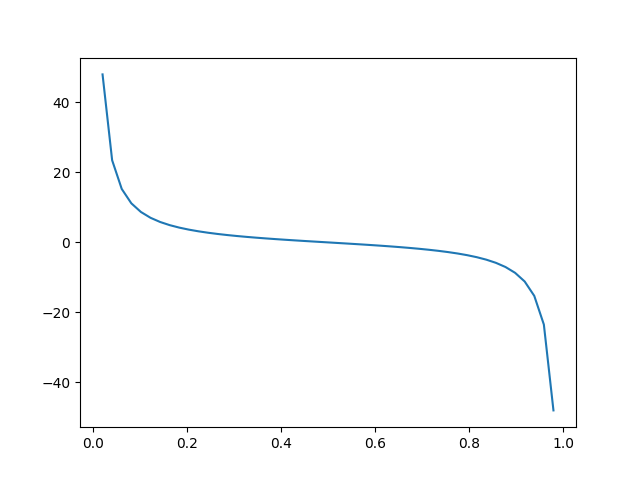
\includegraphics[scale=0.3]{functionofs.png}
\caption{Function $\frac{1}{x}+\frac{1}{x-1}$ on $[0;1]$}
\end{figure}

\end{frame}

\begin{frame}{Analysis}

\begin{alertblock}{Positive invariance}
\begin{theorem}{}
The vector field $f$ of system (\ref{eq:1dtemp}) together with (\ref{eq:sdyn1}) is Lipschitz continuous on $A = [\gamma, 1-\gamma] \times [0;1]$
\end{theorem}

\begin{theorem}{}
\label{posinv}
If $S$ is given by equation (\ref{eq:sdyn1}) and if $a>0$, then the set $A = [\gamma, 1-\gamma] \times [0;1]$ for $\gamma > 0$ sufficiently small is positively invariant for system (\ref{eq:1dtemp}).
\end{theorem}
\end{alertblock}

\begin{exampleblock}{Equilibrium}
\begin{itemize}
\item Only one inside $A : (\frac{1}{2}, \frac{1}{2})$
\item Eigenvalues :
\[
\begin{cases}
\lambda_1 = 0.194602+1.08263i \\
\lambda_2 = 0.194602-1.08263i \\
\end{cases}
\]
\item Stability : Unstable
\end{itemize}
\end{exampleblock}

\end{frame}

\begin{frame}{Poincarré-Bendixson}
\begin{theorem}{Poincarré-Bendixson}
\label{th:pb}
Let $\dx = f(x)$ be a dynamical system with $x \in \mathbb{R}^2$. Let $R$ be a closed bounded subset of $\mathbb{R}^2$ that contains no equilibrium points. Let $t\rightarrow x(t)$ be a trajectory that stays in $R$ for all $t > 0$ and suppose that $f \in C^1$ in an open subset that contains $R$.\\
Then, $x(t)$ is a periodic solution or $x(t)$ tends towards a closed orbit ad $t \rightarrow \infty$.
\end{theorem}

\begin{figure}[H]
\centering
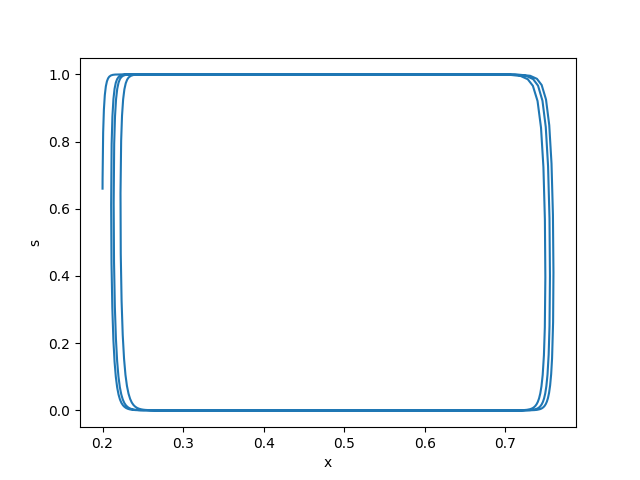
\includegraphics[scale=0.2]{traj1D1_02066.png}
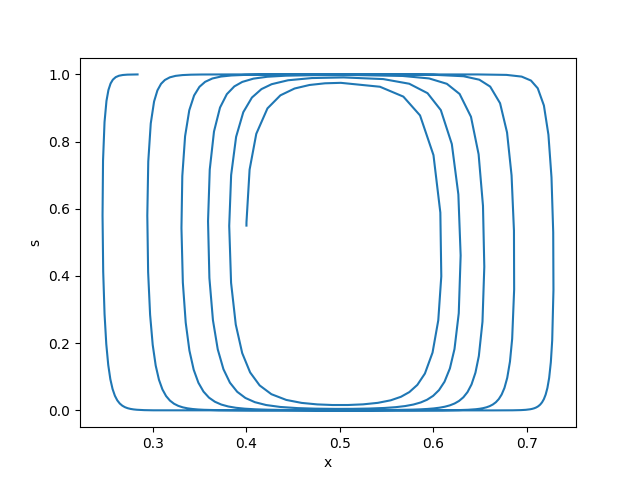
\includegraphics[scale=0.2]{traj1D1_04055.png}
\caption{Trajectories for the system \ref{eq:1dtemp} with status dynamic \ref{eq:sdyn1}. Starting points are respectively $[x_0, s_0] = [0.2, 0.66] \text{   and   } [0.4, 0.55]$.}
\label{fig:traj1D1}
\end{figure}

\end{frame}


\begin{frame}{Second status dynamic}

\begin{equation}
\label{eq:sdyn2}
S(x,s) =  \alpha (\frac{1}{x+1} + \frac{1}{x-2}) (1-s) s
\end{equation}

where $\alpha \in \mathbb{R}_{+}$.

\begin{figure}[H]
\centering
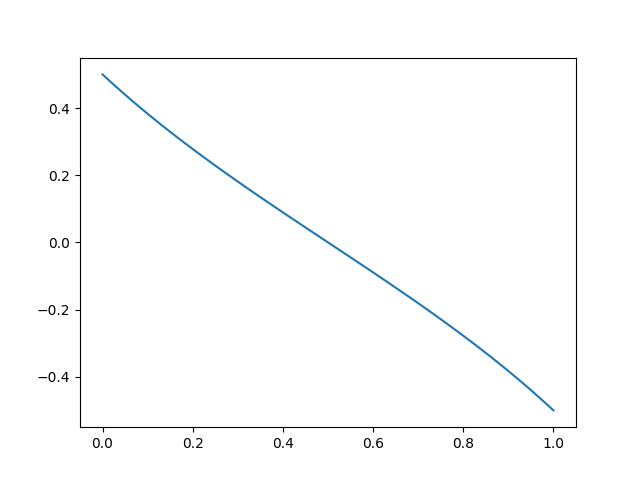
\includegraphics[scale=0.3]{functionofs2.png}
\caption{Function $\frac{1}{x+1}+\frac{1}{x-2}$ on $[0;1]$}
\label{fig:functionofs2}
\end{figure}

\end{frame}

\begin{frame}{Extinction ?}
\begin{figure}
\centering
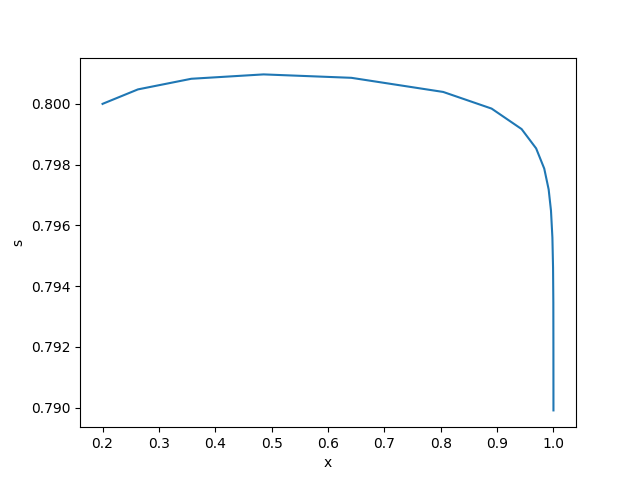
\includegraphics[scale=0.2]{traj1D202081e-3.png}
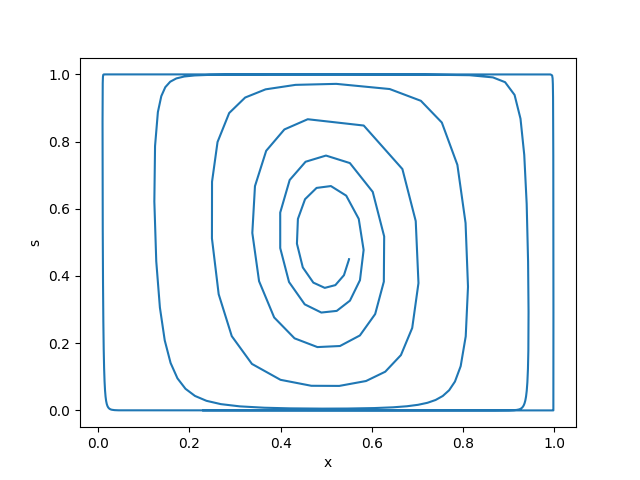
\includegraphics[scale=0.2]{traj1D20550451.png}
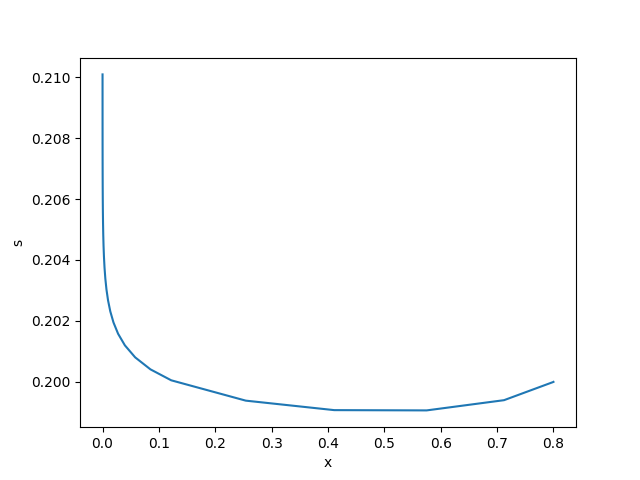
\includegraphics[scale=0.2]{traj1D208021e-3.png}
\caption{Trajectories for the system \ref{eq:1dtemp} with status dynamic \ref{eq:sdyn2}. Starting points are respectively $[x_0, s_0] = [0.2, 0.8], [0.55,0.45] \text{   and   } [0.8, 0.2]$. The value of $\alpha$ is respectively $10^{-3}$, $1$ and $10^{-3}$.}
\label{fig:traj1D2}
\end{figure}
\end{frame}

\begin{frame}{Analysis}

\begin{alertblock}{Positive invariance}
\begin{theorem}{}
\label{posinv2}
If $S$ is given by equation (\ref{eq:sdyn2}) and if $a>0$, then the set $B = [0;1] \times [0;1]$ is positive invariant for system (\ref{eq:bil}).
\end{theorem}
\end{alertblock}

\begin{exampleblock}{Stability}
Nullclines :
$$n_x = \{(x,s) | x=0 \} \cup \{ (x,s)| x = 1 \} \cup \{ (x,s) | sx^{a-1} = (1-s)(1-x)^{a-1} \}$$
$$n_s = \{(x,s) | s=0 \} \cup \{ (x,s)| s = 1 \} \cup \{ (x,s) | x= \frac{1}{2} \}$$
Eigenvalues :
\begin{table}[h]
  \centering
  \begin{tabular}{cccccc}
    & $(0,0)$ & $(1,0)$ & $(1,0)$ & $(1,1)$ & $(\frac{1}{2}, \frac{1}{2})$ \\
    \hline
    $\lambda_1$ & 0.31 & -1 & 0 & -1 & $0.194602+0.310758i$ \\
    \hline
    $\lambda_2$ & 0.5 & -0.5 & -0.5 & 0.5 & $0.194602-0.310758i$ \\
    \hline
  \end{tabular}
\end{table}
\end{exampleblock}
\end{frame}

\begin{frame}{Basin of attraction}

\begin{alertblock}{What does it depend on ? }

\begin{itemize}
\item Strength parameter $\alpha$
\item Intial status $s_0$
\end{itemize}

\begin{figure}[H]
\centering
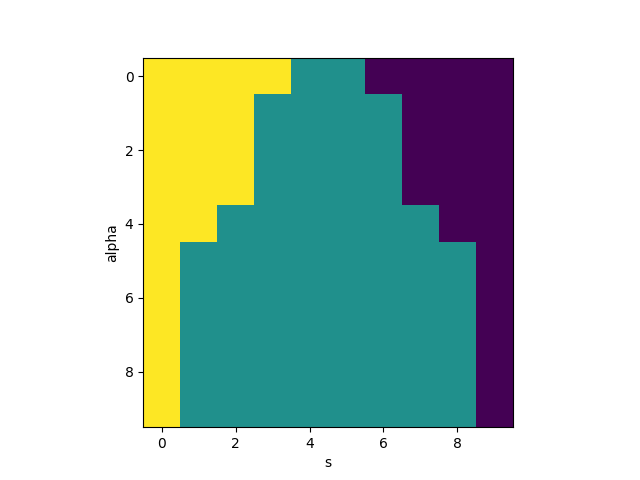
\includegraphics[scale=0.3]{convergence_heatmap.png}
\caption{Heat map of the long term behavior of the system with respect to the initial status and the parameter $\alpha$. In yellow, the trajectories that converged to $(0,1)$. In purple, the trajectories that converged to $(1,0)$. In blue, the trajectories that did not converged to any of the fixed points.}
\label{fig:heatmap}
\end{figure}

\end{alertblock}

\end{frame}

\section{Bilinguism}

\begin{frame}{System}
\begin{equation}
\label{eq:2d}
\begin{cases}
\dx = c(1-x) \Big( (1-k)s(1-y)^a - (1-s)x(1-x)^{a-1} \Big) \\
\dy = c(1-y) \Big( (1-k)(1-s)(1-x)^a - sy(1-y)^{a-1} \Big) \\
\ds = \alpha \Big( \frac{1}{x+1} - \frac{1}{y+1}\Big) s (1-s) \\
\end{cases}
\end{equation}

\begin{exampleblock}{Nullclines}
\begin{figure}[H]
\centering
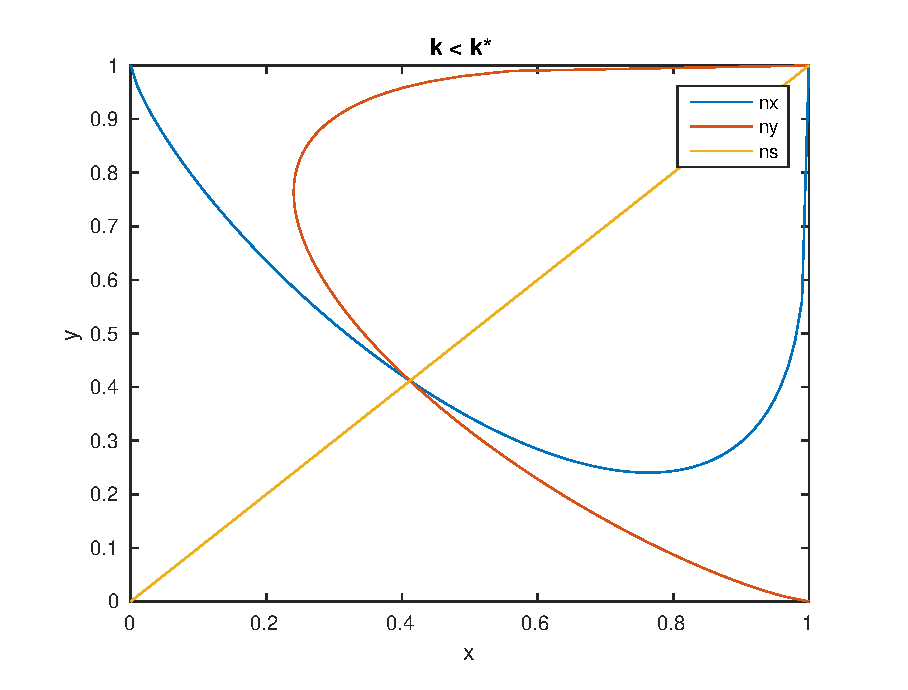
\includegraphics[scale=0.2]{nullpp.eps}
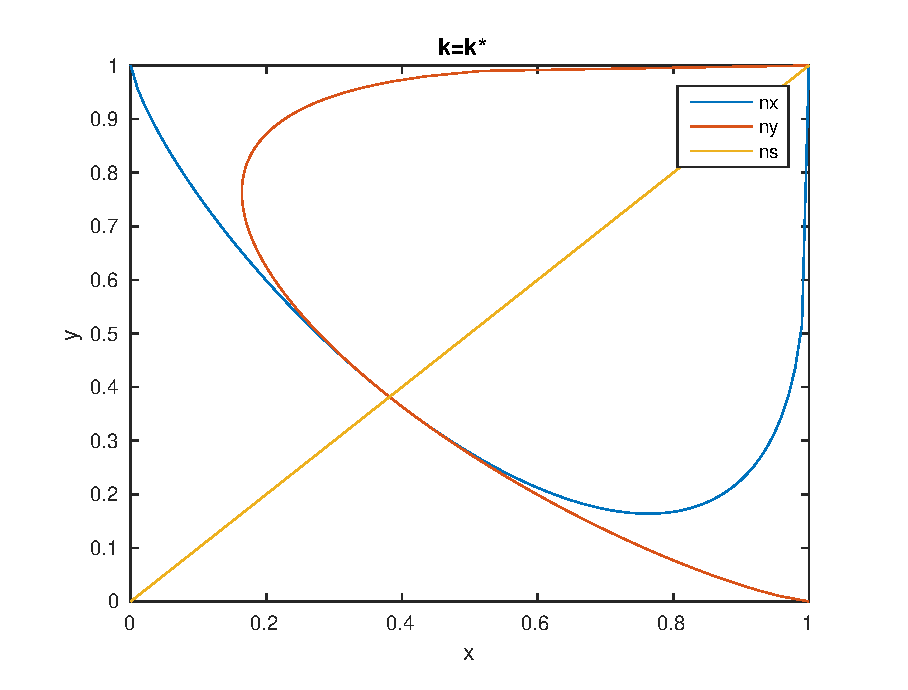
\includegraphics[scale=0.2]{nulle.eps}
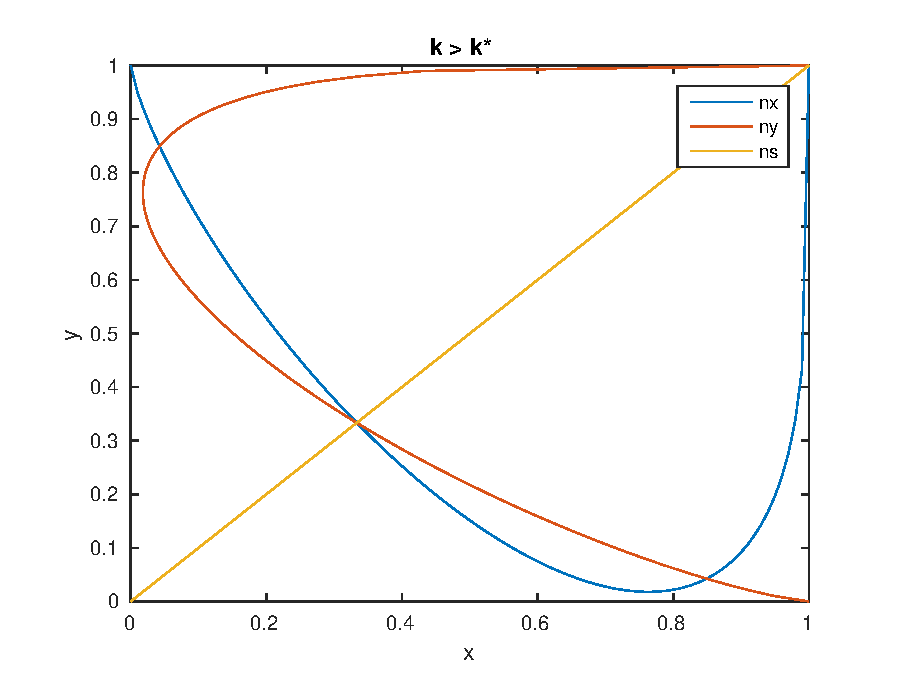
\includegraphics[scale=0.2]{nullpg.eps}
\caption{Nullclines of the system in the plane $s=\frac{1}{2}$}
\label{fig:nullclines}
\end{figure}
\end{exampleblock}
\end{frame}

\begin{frame}{Bifurcation in the new system}

\begin{alertblock}{Coexistence region and numerical simulation}
\begin{figure}[H]
\centering
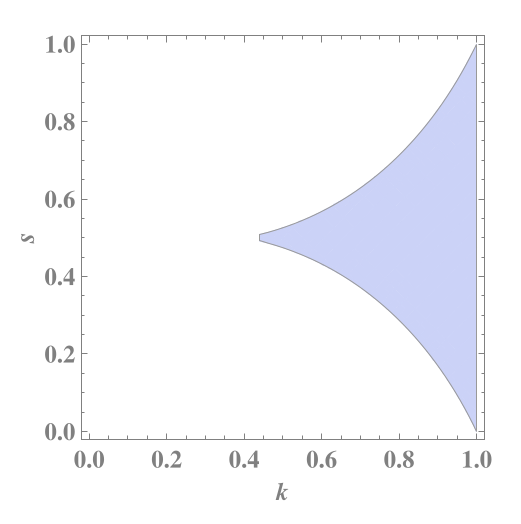
\includegraphics[height=4cm]{coexistence.png}
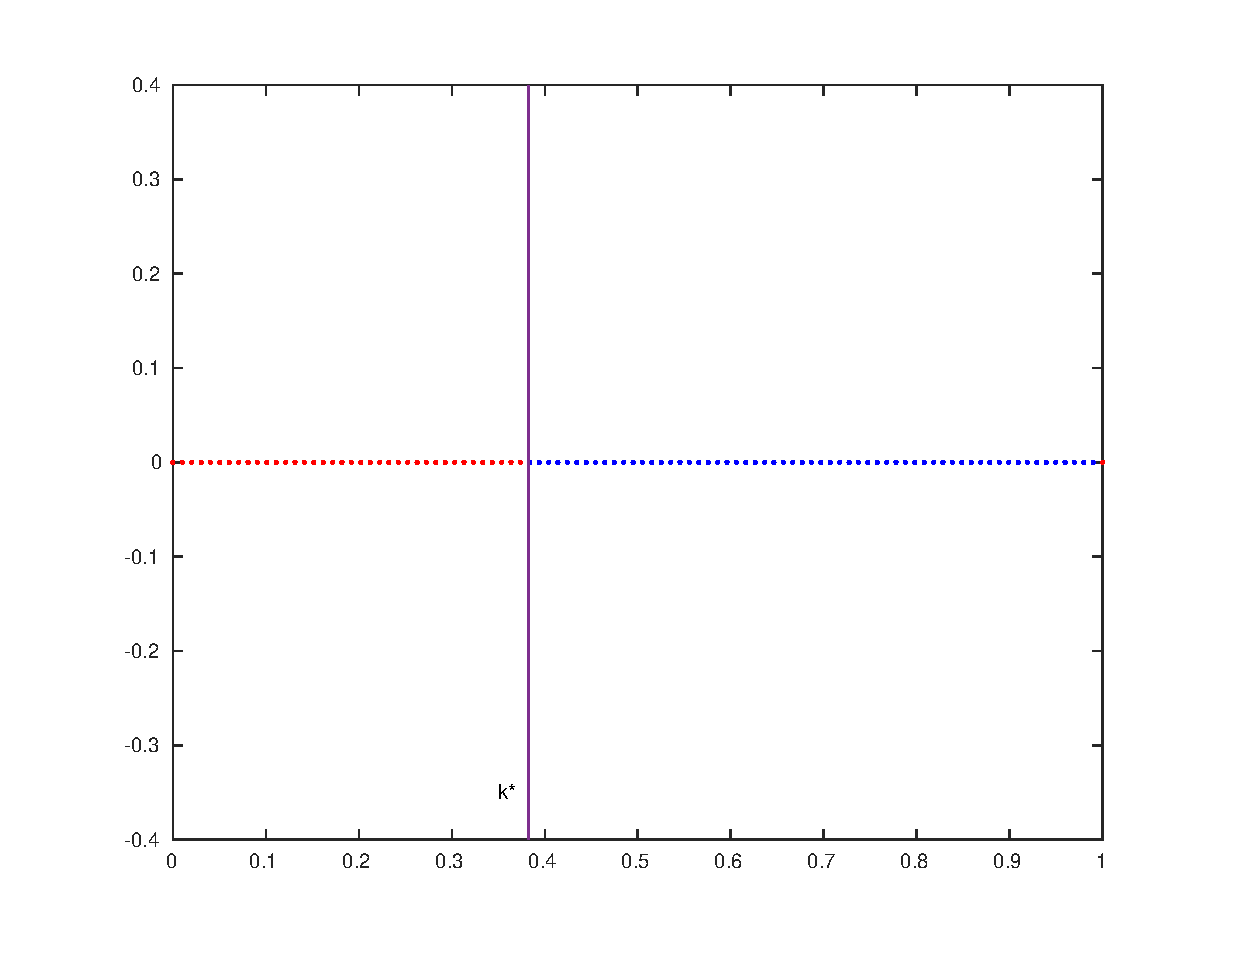
\includegraphics[height=4cm]{bifur.eps}
\caption{(Left) Coexistence region in function of $s$ and $k$. (Right) Numerical simulation of the stability of the equilibrium for system \ref{eq:2d}. Red corresponds to unstability while blue corresponds to stability. The vertical line represent $k=k^{\ast}$.}
\label{fig:coexistence}
\end{figure}

\end{alertblock}

\end{frame}

\section{Spatial analysis}

\begin{frame}{Basics}

\begin{alertblock}{Notations}
\begin{itemize}
\item $K$ regions of similar surface
\item Proportion of $X$ speakers in region $k$ : $x_k$
\item $\mathcal{N}_k(x)$ : mean of $x_i$ in all neighbors $i$ of $k$
\end{itemize}
\end{alertblock}

\begin{exampleblock}{System}
\begin{equation*}
\dx_k = c\big( (1-x_k)s\mathcal{N}(x)^a - x_k(1-s)(1-\mathcal{N}(x))^a \big) \hspace{1cm} \forall k \in \{1,...,K\}
\end{equation*}
\end{exampleblock}

\end{frame}

\begin{frame}{Test on a real dataset : The Irish case}

\begin{alertblock}{Dataset}
\begin{itemize}
\item Region = electoral district
\item Reshape the country into a $135 \times 135$ square for simplicity
\item Suppose no bilinguals (strong)
\end{itemize}
\end{alertblock}

\begin{exampleblock}{Results}
\begin{figure}[H]
\centering
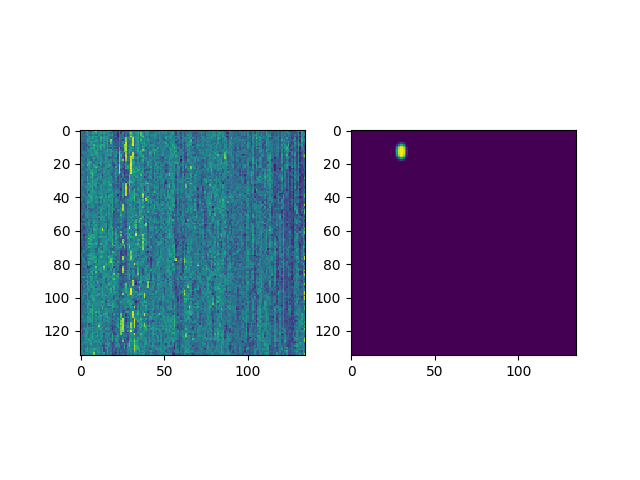
\includegraphics[scale=0.28]{firstandlast_ir.png}
\caption{First and last frame of the simulation of the spatial model.}
\label{fig:firstandlast_ir}
\end{figure}
\end{exampleblock}

\end{frame}

\begin{frame}{Slower dynamics}
\begin{alertblock}{What does it tell us ?}
\begin{itemize}
\item Quickly binary shape
\item The dynamic is slower !
\end{itemize}

\begin{figure}[H]
\centering
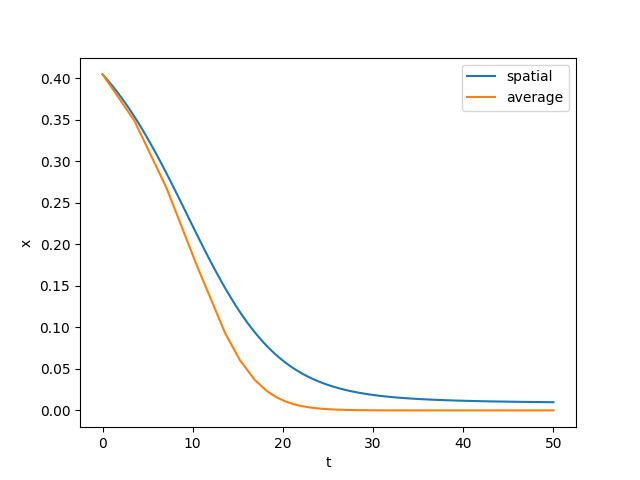
\includegraphics[scale=0.37]{overall_dyn_ir.png}
\caption{Average proportion of Irish speakers throughout the country using both dynamics.}
\label{fig:overall}
\end{figure}

\end{alertblock}
\end{frame}

\section{Conclusion}

\begin{frame}[standout]
    Questions?
\end{frame}

\end{document}
